% !TeX root = ../main.tex
% !TEX spellcheck = en_GB

\chapter{Design}
\label{ch:Design}

\section{Sequence Diagrams}
The sequence diagrams, \crefrange{fig:SD:init}{fig:SD:upload} below, are meant to give an understanding of the inner workings of the \systemName.

Initiation of the system is described in \cref{fig:SD:init}.
It shows the µC initiating itself and then the external blocks.
The GPS module is polled until it returns valid location data. The time returned from the GPS allows the µC to know the time and run the desired actions either at certain intervals, e.g. every 10 minutes, or at specific times, e.g. every full hour.
When valid data has been retrieved it is saved to the SD card and the GPS and GSM modules are put to sleep to conserve power.
The acquisition of GPS location is shown in \cref{fig:SD:getlocation}.
The GPS starts in a sleep mode and is awoken to find it's location.
When the location is found and is valid, the GPS is put back to sleep and the data is saved to the SD card.
To upload data to the server, the GSM must be awoken and data must be retrieved from the SD card, as shown in \cref{fig:SD:upload}.
When the data has been sent the GSM is put back to sleep.

\begin{figure}
	\centering
	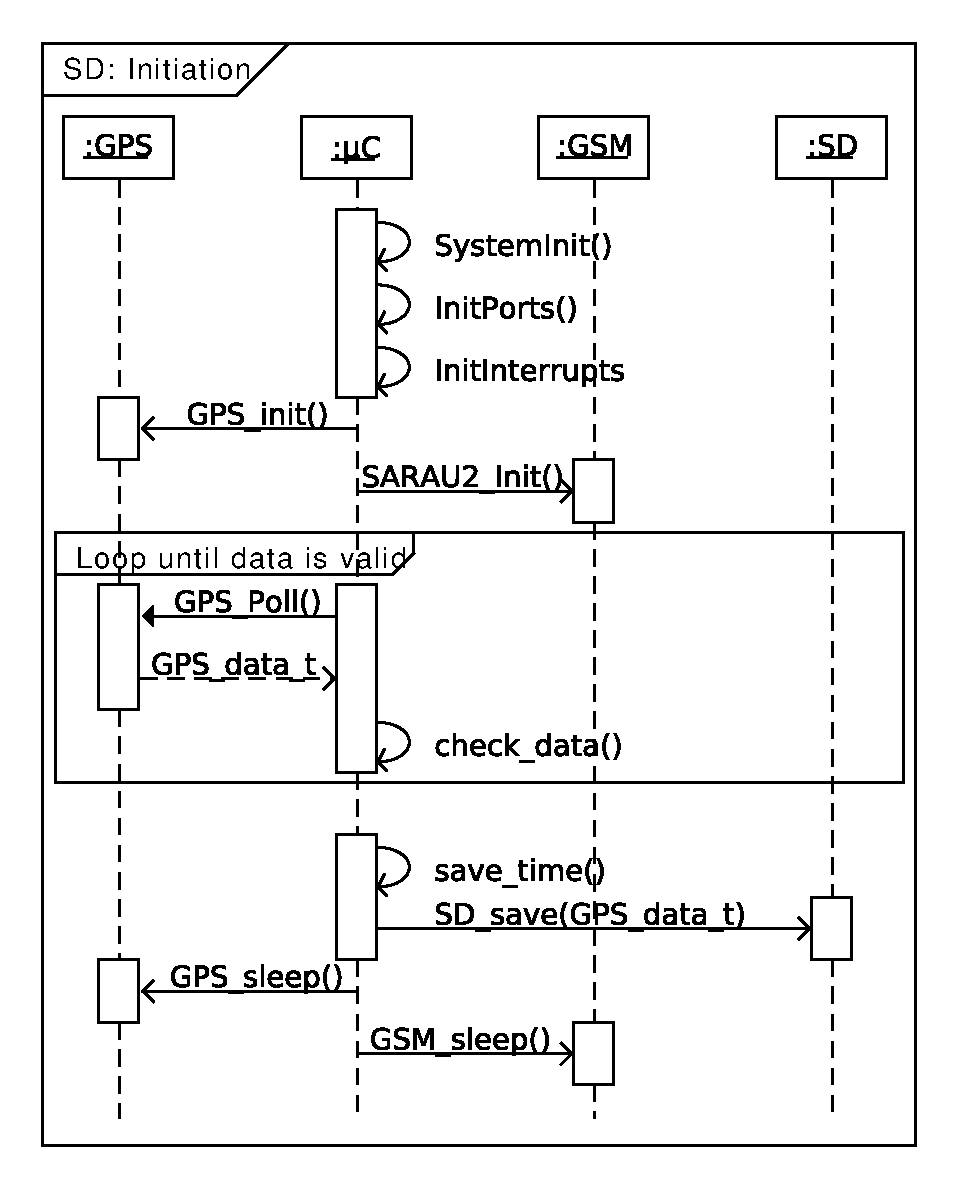
\includegraphics[width=0.7\linewidth]{gfx/Design/SD_init.pdf}
	\caption{Sequence diagram showing the initiation of the system.}
	\label{fig:SD:init}
\end{figure}

\begin{figure}
	\centering
	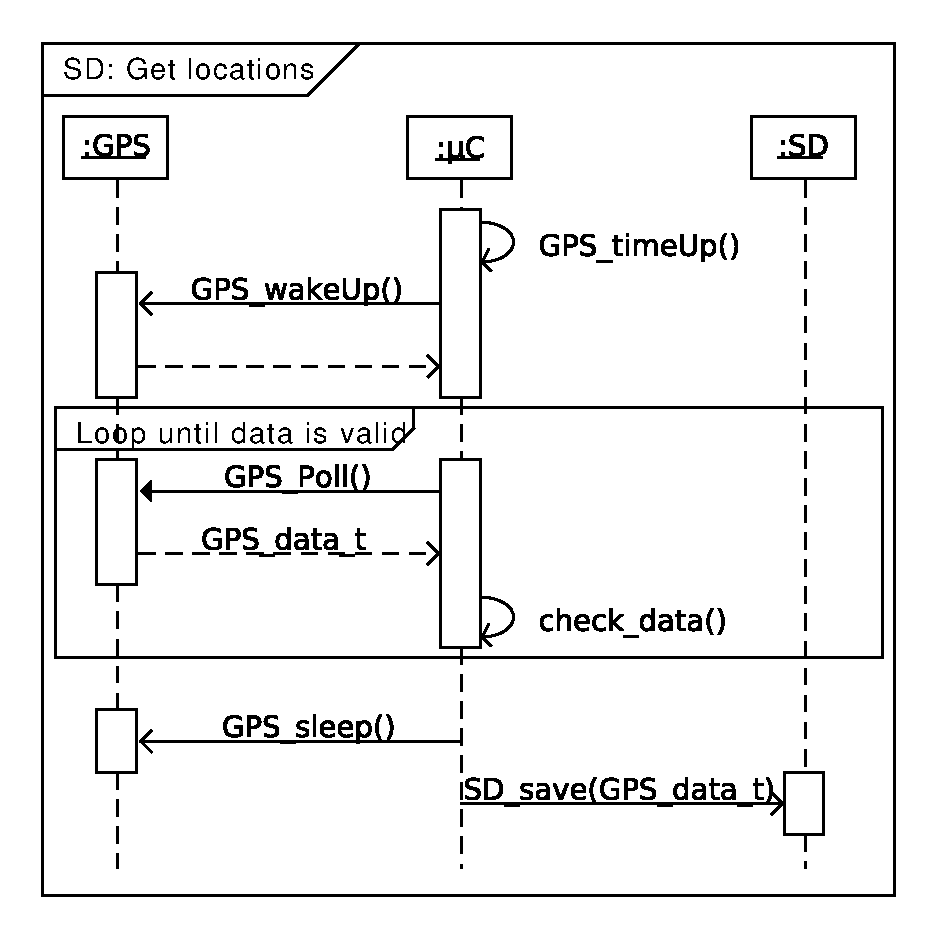
\includegraphics[width=0.7\linewidth]{gfx/Design/SD_getLocation.pdf}
	\caption{Sequence diagram describing the acquisition and saving of GPS data.}
	\label{fig:SD:getlocation}
\end{figure}

\begin{figure}
	\centering
	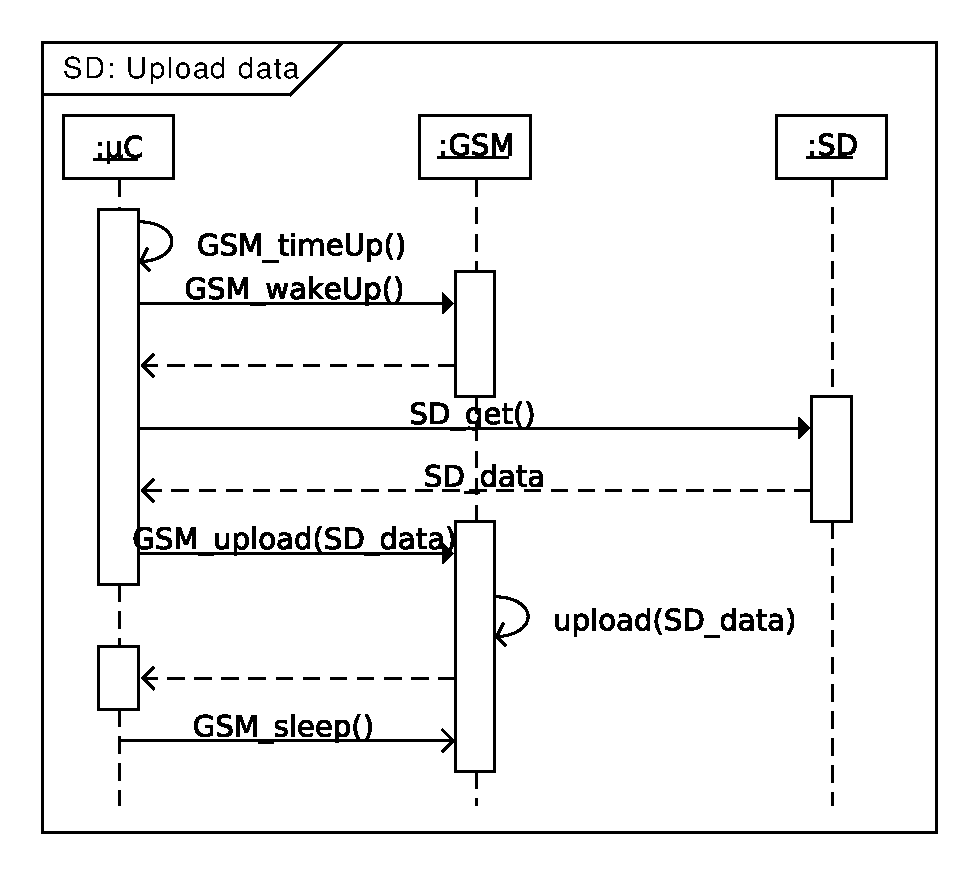
\includegraphics[width=0.7\linewidth]{gfx/Design/SD_Upload.pdf}
	\caption{Sequence diagram showing the process of sending saved data to the server.}
	\label{fig:SD:upload}
\end{figure}

\FloatBarrier
\fxnote{Possible rearranging of this chapter to get UART earlier}
\section{GSM - \SARA}
To facilitate the functionality of the \SARA module, a modem specific driver will be developed. This driver will contain functions to configure \SARA for sending and receiving data through UDP packets.
\fxnote{State diagram?}

\subsection{UART}
Communication with the \SARA module, will be done through a UART connection. The module contains an ability to auto detect the baud rate of the first transmission, and use this baud rate to respond. In addition it supports the standard baud rates: \num{1200}, \num{2400}, \num{4800}, \num{9600}, \num{19200}, \num{38400} and 5 higher rates. \num{9600} baud was selected with focus on stability and the ability to debug the communications.

\subsection{AT Command Interface}
Through the application a limited amount of commands is necessary, the command flow is displayed on \cref{fig:SD:configConnection}. While functionality of the commands used are described, in \cref{app:sarau201}.

\begin{figure}
	\centering
	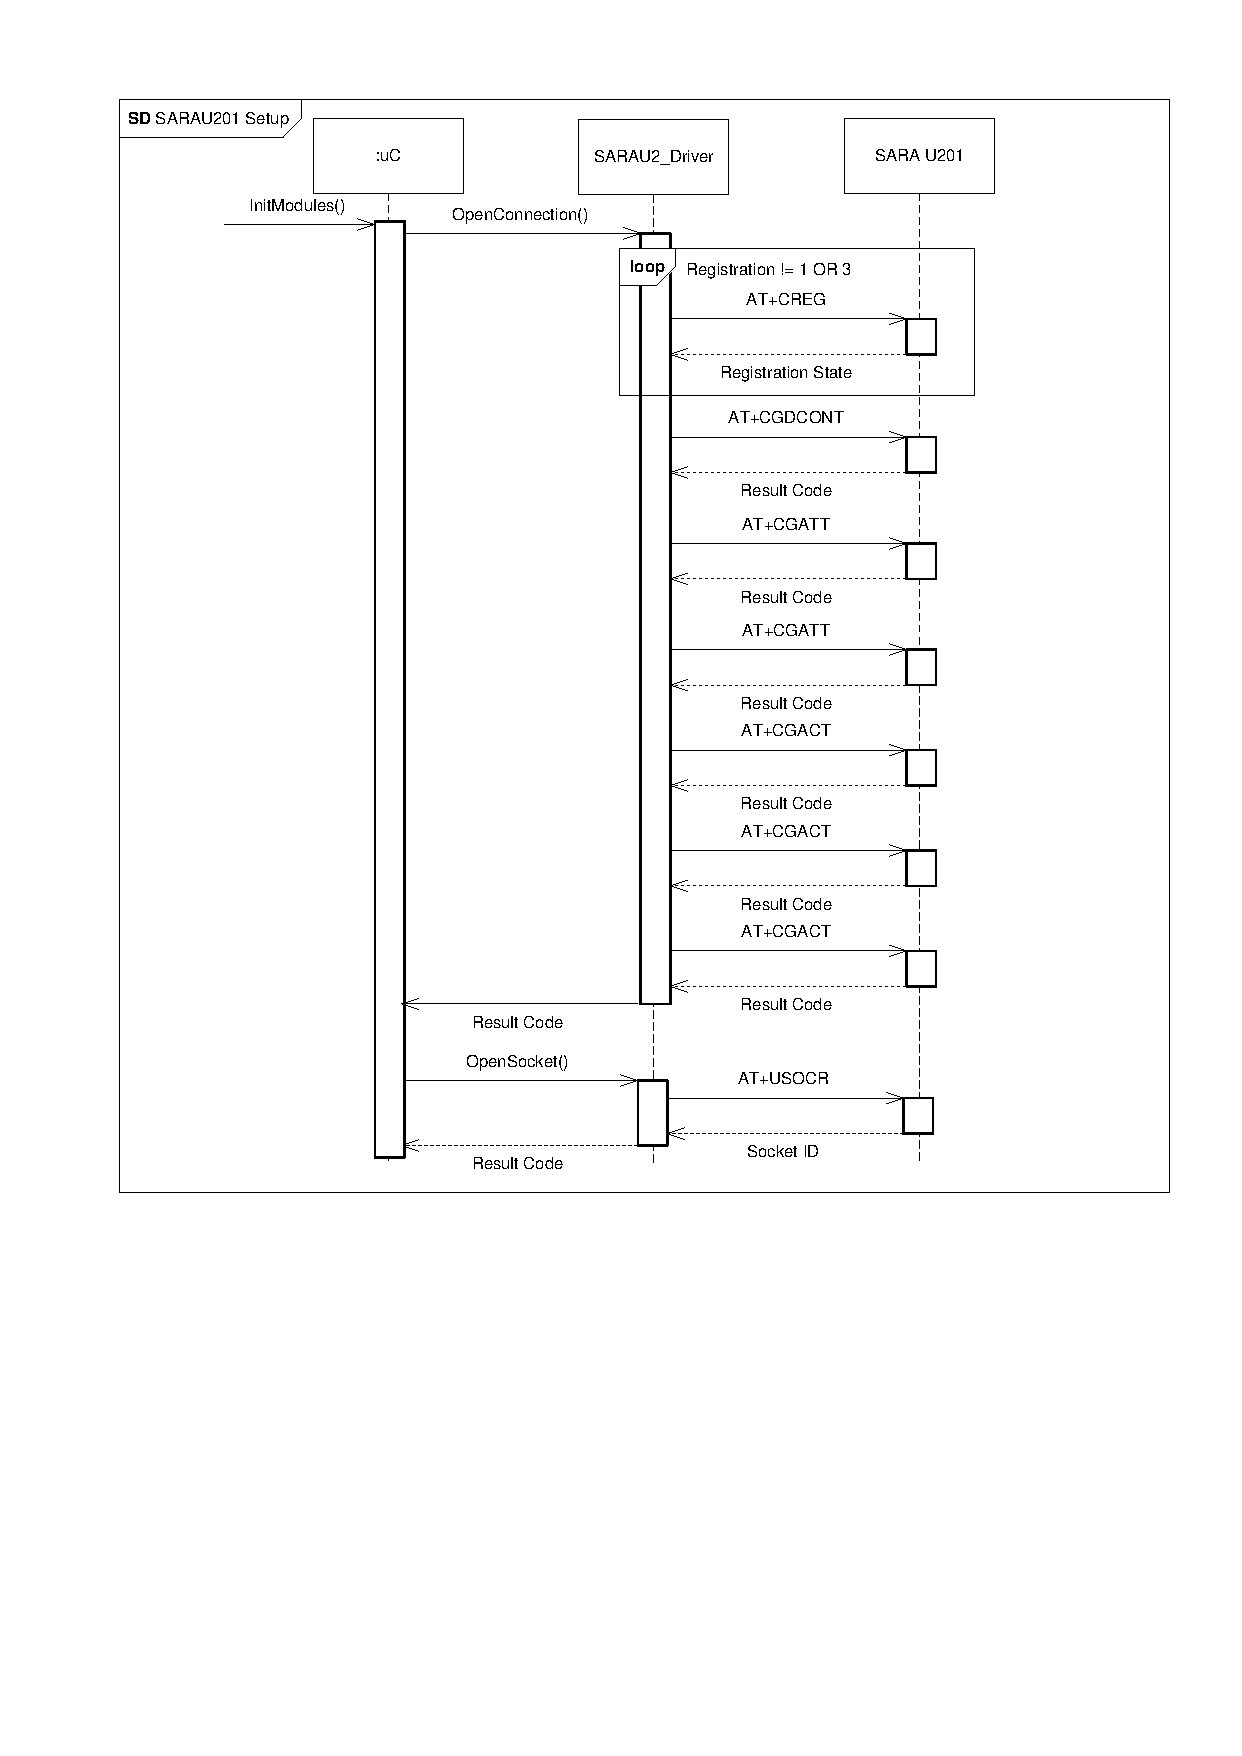
\includegraphics[width=0.9\linewidth, clip, trim={2cm 9cm 1cm 1cm}]{gfx/Design/GSMSetupConnection.pdf}
	\caption{Sequence diagram of AT configuration of \SARA module.}
	\label{fig:SD:configConnection}
\end{figure}

Noteworthy in \cref{fig:SD:configConnection} is, the calls between SARAU2 Driver and SARA U201 should be seen as UART transmissions, and not direct method calls. The transmission is facilitated by the an UART driver. 

\section{GPS - \GPS}
The design of the GPS is shown as a flow diagrams in figures~\ref{fig:gpsflowsend} and \ref{fig:gpsflowfindheader}.
After an initiation is run for the GPS module, it only returns data when something is sent to it.

As seen in \cref{fig:gpsflowsend}, the first two steps construct the message according to the protocol described in \cref{sec:UBXprot}.
Then the message is sent, and the response header is located in the UART buffer, as shown in \cref{fig:gpsflowfindheader}, where every unused byte before the header is removed with the \mintinline{c}{popByte()} function.
When the received data has been located, the first six bytes, including the length of the payload are loaded, and the type of message is determined.
If the response is an ACK, the program can continue, but if it is a NACK, the message has to be sent again.
If the response contains GPS\_data, the data must be read, interpreted and saved to the SD-card.

\begin{figure}
	\centering
	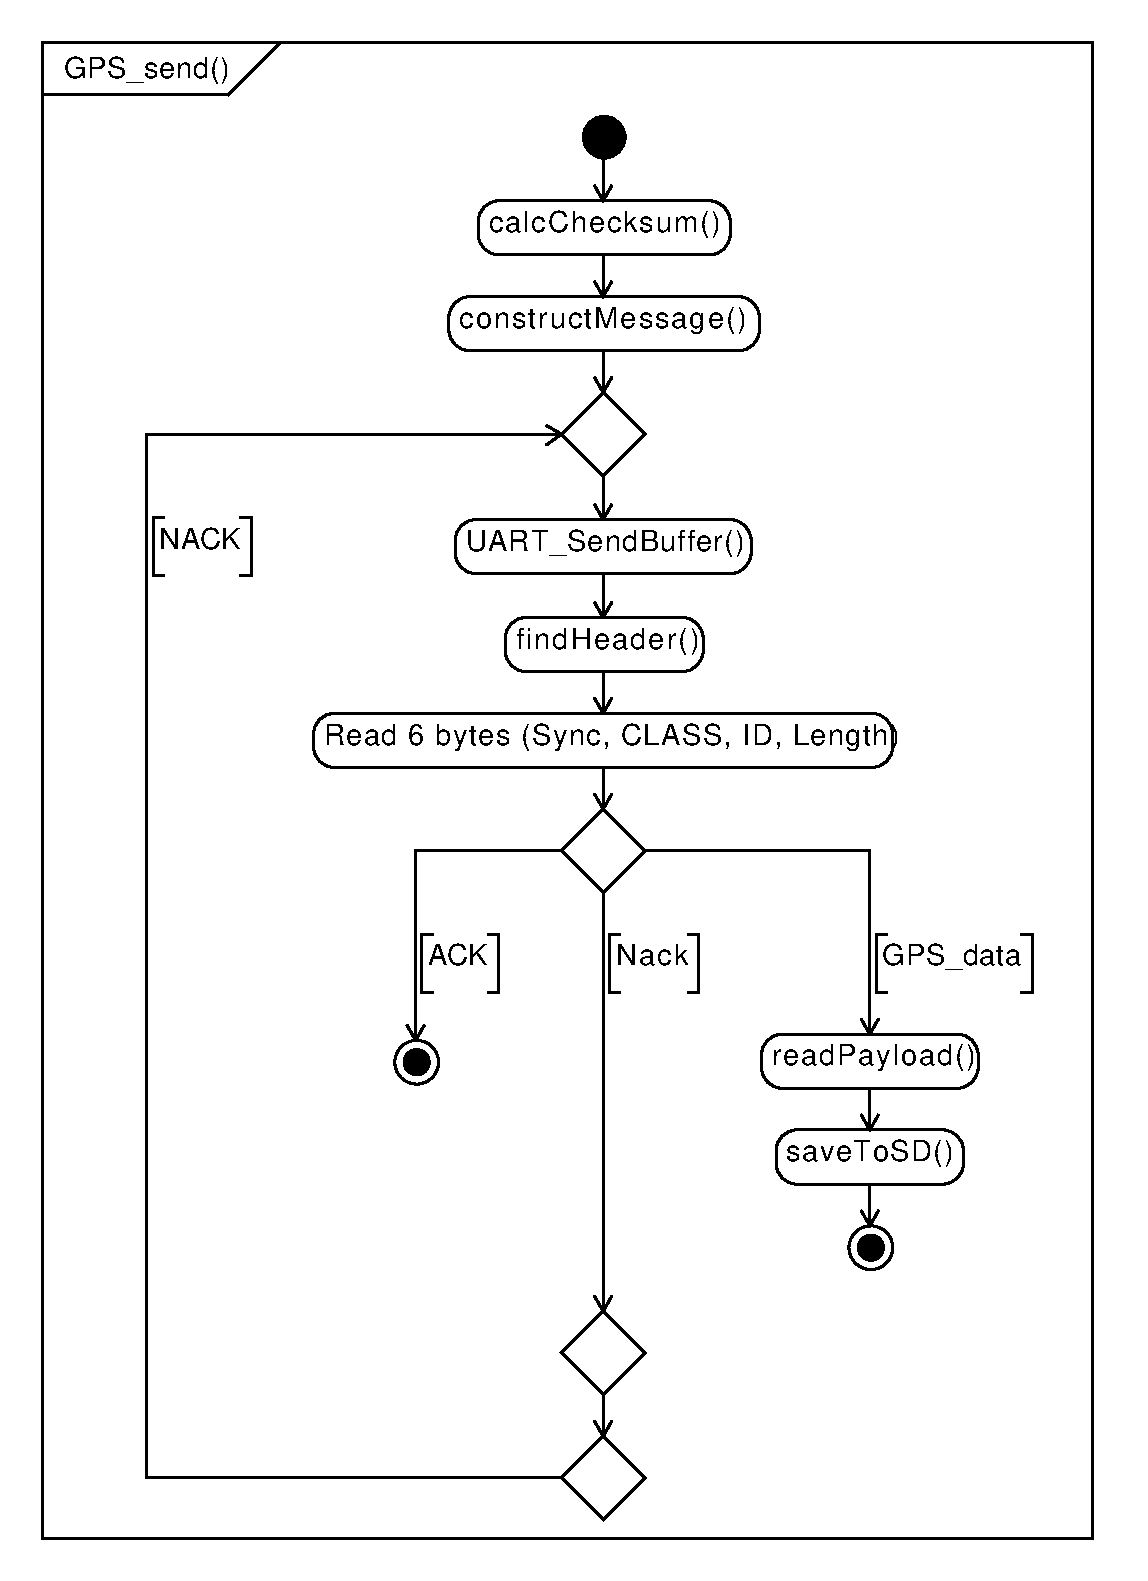
\includegraphics[width=0.7\linewidth]{gfx/Design/GPSFlowSend.pdf}
	\caption{Flow diagram for \mintinline{c}{GPS_send()}.}
	\label{fig:gpsflowsend}
\end{figure}

\begin{figure}
	\centering
	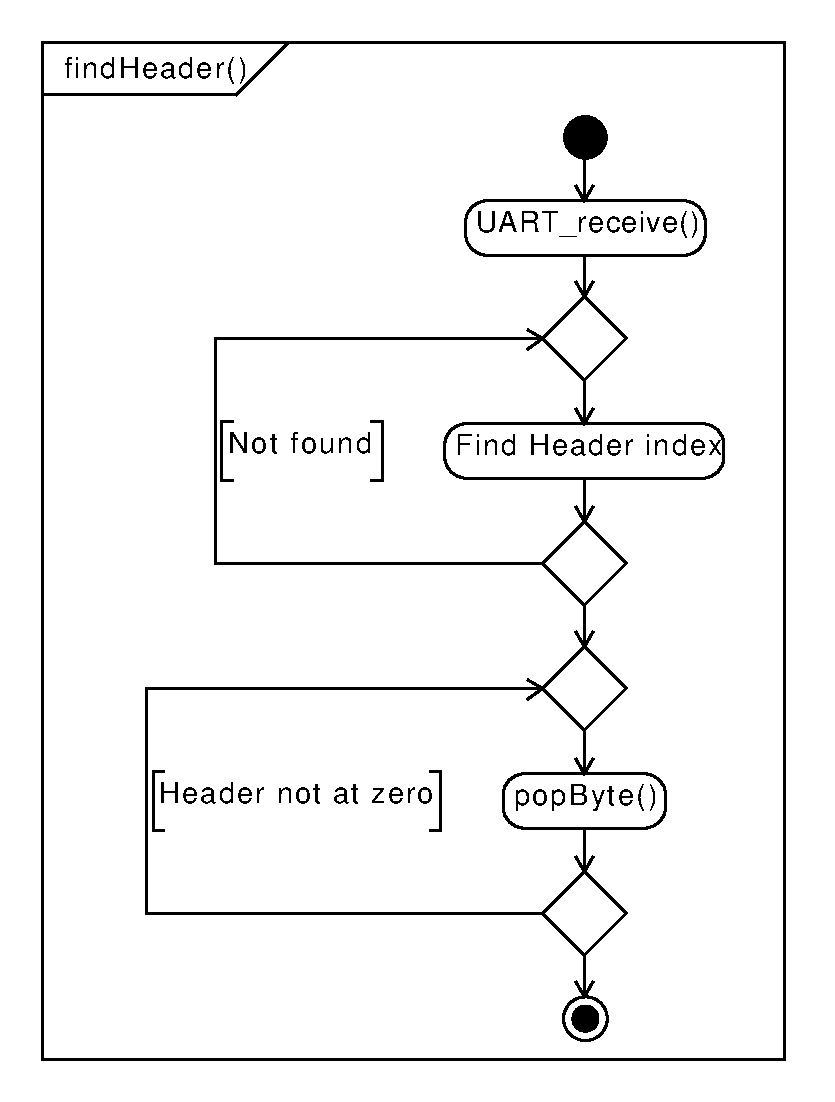
\includegraphics[width=0.7\linewidth]{gfx/Design/GPSFlowFindHeader.pdf}
	\caption{Flow diagram for \mintinline{c}{findHeader()}}
	\label{fig:gpsflowfindheader}
\end{figure}

\fxnote{Choices + Diagrammer}

\section{SD-card - \SDsock}
The SD-card is to be used without a file system, as the stored data will be hex values of known size.
The necessary functions to write will be
\begin{minted}{c}
	uint8_t SD_save();
	GPS_data_t SD_load();
	uint8_t SD_delete();
\end{minted}
where \mintinline{c}{GPS_data_t} is a struct containing the time and location of a given GPS data point.
\mintinline{c}{SD_delete()} is meant to delete any data points already sent to the remote server.

\section{Controller - \SAMD}
General flow of the system is linear, where the modules are initialise. And the gps polling is looped. 
But since the communication protocols are asynchronous, it was decided to make the serial ports interrupt based. Meaning that the main thread will not prevent data from being sent or received. While also making the send and receive functions non blocking.

\subsection{UART - BaudRate}
Both \SARA and \GPS supports the usage of auto baud rate detection, meaning that they will respond to a message in the same baud rate as they receive.
But due to consistency, both modules is set to the selected baud rate during their set up configuration. 
For simplicity a baud rate of \SI[per-mode = symbol]{9600}{\bit\per\second} was chosen, specification for the UART is shown in \vref{tab:BaudRate}.

\begin{table}[H]
	\begin{tabular}{ll}
		\hline 
		Baud Rate & 9600 \\ 
		\hline 
		Data Bits & 8 \\ 
		\hline 
		Parity & None \\ 
		\hline 
		Stop Bits & 1 \\ 
		\hline 
	\end{tabular}
	\centering
	\caption{Baud rate definition used for serial com ports on \SAMD.}
	\label{tab:BaudRate}
\end{table} 

\FloatBarrier